\documentclass[10pt]{article}
\usepackage{latexsym}
\usepackage{algorithm}
\usepackage{algpseudocode}
\usepackage{natbib}
\usepackage{graphicx}
\usepackage{subfigure}
\title{Action Selection in ASAMI}
\date{}

\linespread{1.5}

\begin{document}
\maketitle

\begin{abstract}
Robot motion planning and control is essential for robots to navigate
in the real world.
Autonomous robots are expected to take actions to actively explore an
environment, instead of fed by hand-tuned knowledge given by human.
Stronger and Stone designed an algorithm, called ASAMI, which
developes the learning efficiently. This assumes prior domain
knowledge of the effect of the actions. However, we may not have
access to this information in some domains. I proposed an extension on
ASAMI which makes it overcome such drawback, to learn the actions and
also the envrionment simutanously.
\end{abstract}

\section{Introduction}

There are two critical models for robot motion---action model and
sensor model. The action model predicts the effect of an action,
or formally, $A \rightarrow \Delta S$, where $A$ is the action space
and $S$ is the location space. The sensor model predicts the
location given an observation, or formally, $O \rightarrow S$, where
$O$ is the observation space. Traditionally, these two models are
given by human. The robot only needs to do planning or learning for a
higher-level goal (Figure~\ref{fig:robocup}).

\begin{figure}
\centering
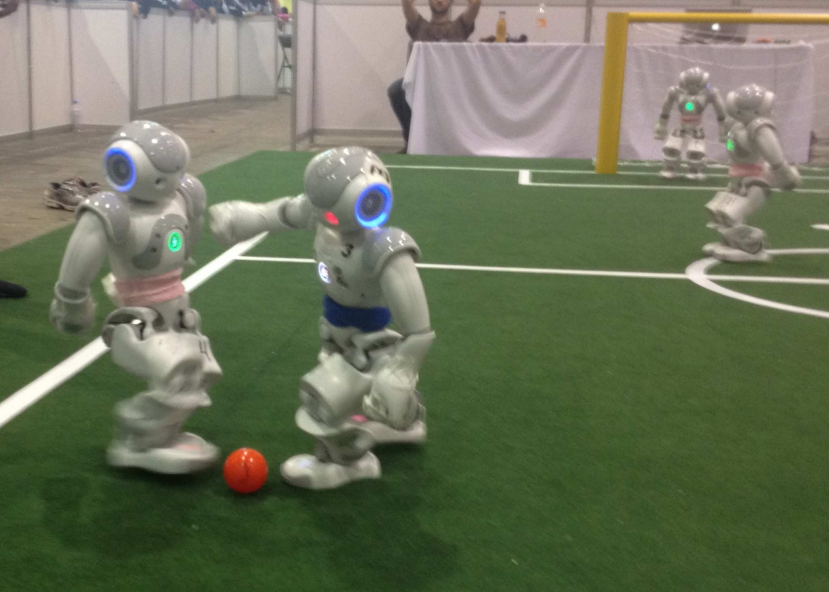
\includegraphics[width=0.7\columnwidth]{Robocup.png}
\caption{Robots play soccer. \cite{LNAI12-Barrett}}
\label{fig:robocup}
\end{figure}

However, robots can be learn action model and sensor model
simultaneously without any prior knowledge. One example is the ASAMI
algorithm \cite{CSJ06}. There are two estimates of the current state
of the robot --- $W_s$, the state estimated by the sensor model, and
$W_a$, the state estimated by the action model. They are both assumed
to be polynomial functions. The robot needs to estimate the parameters
of them. In one ASAMI iteration, the action model is used to update
the sensor model, and also vice versa. This is called bootstrapping.
This idea is illustrated in Figure~\ref{fig:relation}.

\begin{figure}
\centering
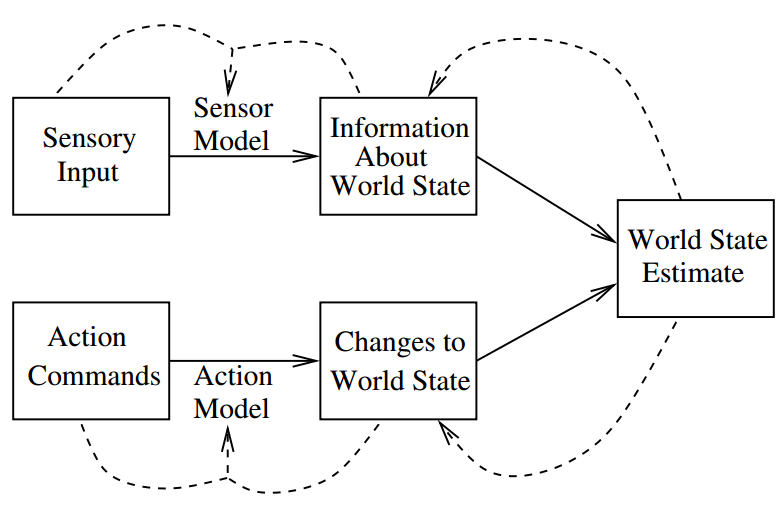
\includegraphics[width=0.7\columnwidth]{relation.png}
\caption{the robot can use redundant information to learn its action
and sensor models, revised from Figure~2 in \cite{CSJ06}.}
\label{fig:relation}
\end{figure}

\section{Analysis of ASAMI}

In ASAMI, actions are selected randomly
in the training. However, this can be biased according to the current
belief.  In this sense, the agent should be able to determine which
action would lead to the most uncertain results and thus need more
samples.  The agent doesn't know the correctness of the models. It
only knows the consistency of them. For example, states with larger
difference in action model and sensor model ($|W_a - W_s|$) should be
considered as inconsistent.  Unobserved state, action pairs can be
also assumed to be inconsistent.

The first author of \cite{CSJ06}, Dan Stronger, commented that ``one
possible reason the $W_a$ is wrong after a certain action is that the
action is just very noisy \ldots This is a good reason to gather more
data for that action \ldots  But another possible reason  an action
could be causing problems is because the action model function being
fit, with the degrees of freedom that it has, just fits to a function
that's not especially accurate for that action''. This would be a
problem in degree selection in the polynomial regression
\cite{IJAIT08-stronger}. In this paper, I'll give our action model
proper degrees of freedom. So, if the action model is inconsistent,
the reason should be that either there are too few data gathered to
make consistency happen, or the data gathered are too noisy.

Action selection is even necessary in some environment. The
experiments in \cite{CSJ06} assume that \textit{we} know the effects of
the actions -- for example, some actions would make the robot go
forward, and others make it go backward -- while the robot does not
know.
So to explore the environment, we make the robot walk forward and
backward alternatively to explore the state space. However, 
actions' effects may be completely unknown.  If the agent still chooses the
actions uniformly random, then exploration would be inefficient.

For example, we consider one-dimensional walk. Let the world be in the
range of $[0,n]$. The agent starts at 0, and wants to reach $n$. Let
the range of velocity be $[-2a, 2a]$ (positive velocities mean going
forward, and negative ones mean going backward), and in every step the
agent chooses an action uniformly random.  Then, the expected absolute
velocity is $a$. Assume the agent would ``bump into'' the boundary of
$0$ and stays there if it tries to go backward from position $0$. The
expected \textit{moving forward} steps needed to take to reach
position $n$ from $0$ is $\frac{n}{a}$. This forms a \textit{random walk}
\cite{motwani1995randomized} problem. The expected steps needed to
take to reach distance $n$ is $O(n^2)$. This implies that, if an
agent takes random actions in an unknown domain, it is likely that the
agent would restrict itself in a small sub-domain.

\section{Literature Review}

In the perspective of model-adaptive agents \cite{maes1993modeling},
\textit{action selection} is critical problem because it
accelerates the progress towards its goal---consistency between action
model and transition model. This also solves the problem of
\textit{learning from experience}, as the inconsistency is an
essential information that can be used for further decision-making.

There is a two-dimensional version of ASAMI discussed in
\cite{ICRA08-stronger}.  As the action space is larger in higher
dimension, biasing on actions instead of random selection on actions
becomes more essential.

Compared with this proposed method, some similar ideas are discussed
in the developmental robotics literature. They call the inconsistency
described above as \textit{error} \cite{oudeyer2006discovering},
\textit{surprise} \cite{ranasinghe2008surprise} or \textit{curiosity}
\cite{schmidhuber2006developmental}. This serves as a motivation to
change the model. A metric can be used to describe the global
inconsistency \cite{oudeyer2006discovering}. Then, a reinforcement
learning framework can be used to plan to get to the states with the
least global inconsistency. The authors in
\cite{ranasinghe2008surprise} used logic rules as the model, and let
the robot figure out why there could be a surprise. In this paper, I
assume that the surprise is caused by insufficient or noisy data. So
the surprise, or inconsistency, of an action, is simply caused by the
data gathered at that action.

Additionally, there is an assumption in \cite{CSJ06} that there is a
mapping from action to the difference of state, i.e., $A \rightarrow
\Delta S$, where $A$ is the action space and $S$ is the state space.  This
is true in robot motion. So it's possible to learn the difference of
the states, when an action is given. This is
exactly how the task is designed in \cite{ICDL10-hester}. If this is
not true, so that $S \times A \rightarrow S$ is the best we can
estimate, this would become more challenging but still possibly to be
dealt with. We might know that a certain $(s, a)$ is inconsistent and
we want to gather more data on it. But our action model might not be
well-learned. So the reward should be a compromise between the
inconsistency of that $(s, a)$ and the cost to reach it.

There are also other related works on learning the action model. But
they're using very different approach. They assume that one model,
usually the sensor model, is well calibrated. The data are represented
as either statistics \cite{And_learningand} or instances
\cite{LNAI2007-ahmadi}. These would be further analyzed and compared
with our approach in Section~\ref{sec:dis}.

\section{Proposed Algorithm}

\begin{algorithm*}
\caption{Strong ASAMI}\label{alg:asami}
\begin{algorithmic}[1]
\Function{initialize}{$rangeOfActions$}
    \State $trials\gets 0$
    \State $actions \gets$ discretized $rangeOfActions$
    \For{$action$ in $actions$}
        \State $samples[action] \gets \{\}$ \label{asa:actInit}
	\Comment{Initialize a sample set for each action}
        \State $s \gets A_0(action)$
	\State push $s$ to $samples[action]$
	\Comment{add the prediction by the initial action model}
    \EndFor
\EndFunction
\\
\Function{update}{$action, \Delta state$} \label{asa:update}
    \State add $\Delta state$ to $samples[action]$
    \State increase $trials$
\EndFunction
\\
\Function{getAction}{} \label{asa:getAct}
    \If {$trials\leq$ ACTION\_LEARNING\_TRIALS}
        \State $action \gets$ the action such that $samples[action]$ has the largest variance
    \Else
        \State $action \gets$ appropriate action for state exploration \label{asa:actSel2}
    \EndIf
\EndFunction
\end{algorithmic}
\end{algorithm*}

In this section, I propose an algorithm, which I call it Strong ASAMI,
that makes the agent choose actions in a computationally cheap way.
It keeps the essentials of ASAMI\@. However, Strong ASAMI can be applied
when there is no prior domain knowledge about the action model. The
idea is that we divide the learning process into two phases. The agent
learns the actions first and learns the state space later. In the
first phase, it chooses the action with least confidence to learn. In
the second phase, it uses the actions it learned to explore the
environment.

Some essential functions are presented in Algorithm~\ref{alg:asami}.
In initialization, a sample list is initialized for each action
(Line~\ref{asa:actInit}). $A_0$ is the initial action model (a roughly
correct action model we have), and its prediction for each action is
pushed to the corresponding sample list.  This is a useful
initialization, as the variance of the sample list would represent
the error of our initial model, when the first observed sample is
added.

In each iteration, \texttt{update} (Line~\ref{asa:update}) is called to update
the knowledge of the action effects by adding new observations. When
the robot needs to decide which is the next action to take,
\texttt{getAction} (Line~\ref{asa:getAct}) is called.

The action selection strategy in phase 2 (Line~\ref{asa:actSel2}) is
quite vague. However, this is up to the agent how to plan to traverse
the state space. Consider a one-dimensional environment, it might want
to keep trying actions with positive $\Delta state$. When it observes
no state changes after executing such action, then it tries actions
with negative $\Delta state$. Then the robot should have the
performance of walking forward and backward in the domain.

\section{Experiments}

The plan for the experimental evaluation is designed in the following
way, the robot can walk back and forth in a one-dimensional path.
There is a beacon placed at one end. The robot is always facing
towards the beacon. The only observation is the height of the beacon.
The environment could be noisy - this is inherently tree when doing
experiment on real robots like Nao.

First, I test ASAMI in a toy domain. I only naively implemented the action
model and the sensor model. Then, I made ASAMI and Strong ASAMI work on
Aldebaran Nao robot. Action model and sensor model are both assumed to be cubic
functions.  We have four parameters to estimate for each model. The
initial action model $A_0$ is defined to be a constant function,
$A_0(x) = c$, where c is a small random number. This is used to train
the state estimated by the action model, $w_a$, in the first 100
iterations.

\subsection{Test in Simulator}

\begin{figure}
\centering
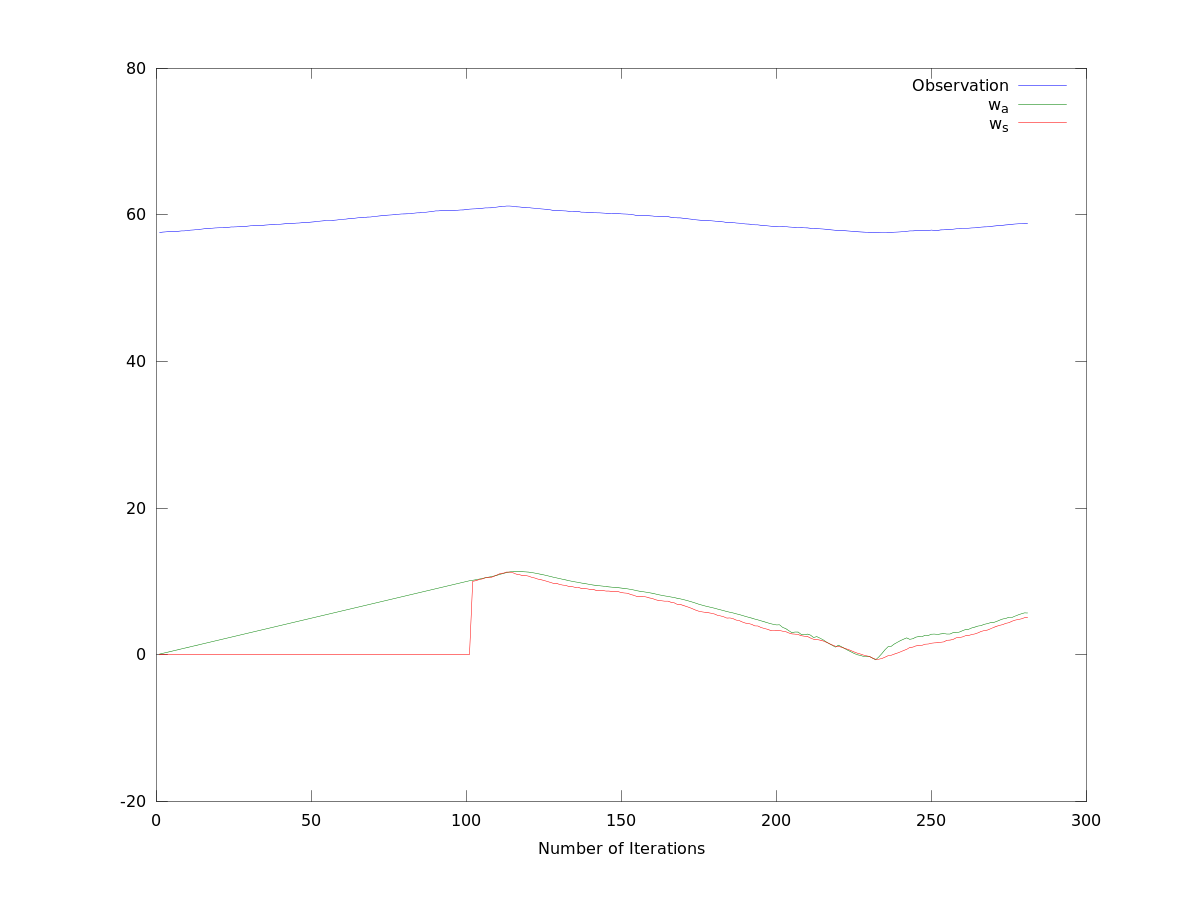
\includegraphics[width=0.7\columnwidth]{simResult.png}
\caption{The learning performance in the simulator.}
\label{fig:sim}
\end{figure}

The actions in the simulator are simply walking backward or froward.
It can choose from velocity of [-1, 1]. The effect of the velocity is
exactly the change of state.
The sensor model computes the height of the beacon according to the
current state. As there is no noise in the simulator, the results show
that learning on both models converge quickly and nicely. The result
is in Figure~\ref{fig:sim}.

\subsection{Test on Nao: First Attempt}
\label{nao:1st}

The challenges of making ASAMI walk on Nao are that beacon height is
too noisy. The height returned by the beacon detector could be noisy,
as the observed image can be blur. The real walking velocity can be
different from what is set. The result is in Figure~\ref{fig:demo}.

Observation is retrieved and ASAMI is updated in each iteration. It
can be told from the beacon height that the robot walks forward and
backward two times, and then kidnapped from a further point to a
closer point to the beacon in around 3,500 iteration.

\begin{figure}[h]
\centering
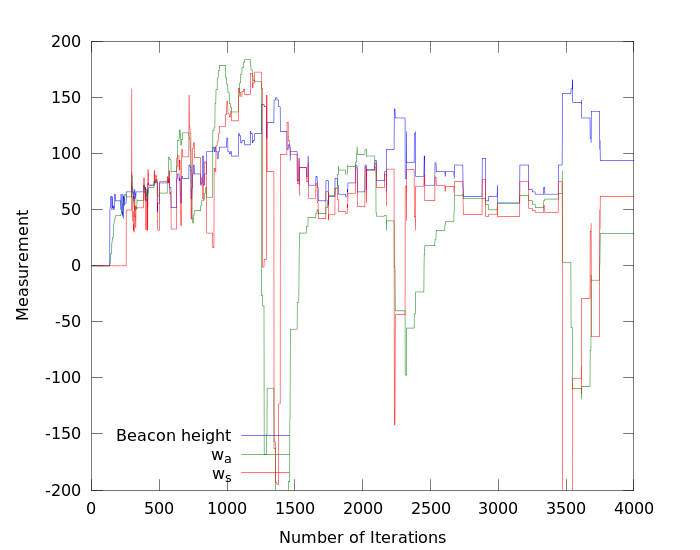
\includegraphics[width=0.7\columnwidth]{demoResult.png}
\caption{Testing of ASAMI on Nao during the class demo. The
observation comes continuously, on average of 30 frames (iterations)
per second. It is kidnapped at around 3,500th iteration.}
\label{fig:demo}
\end{figure}

\subsection{Test on Nao: Second Attempt}

\begin{figure}[h]
\centering
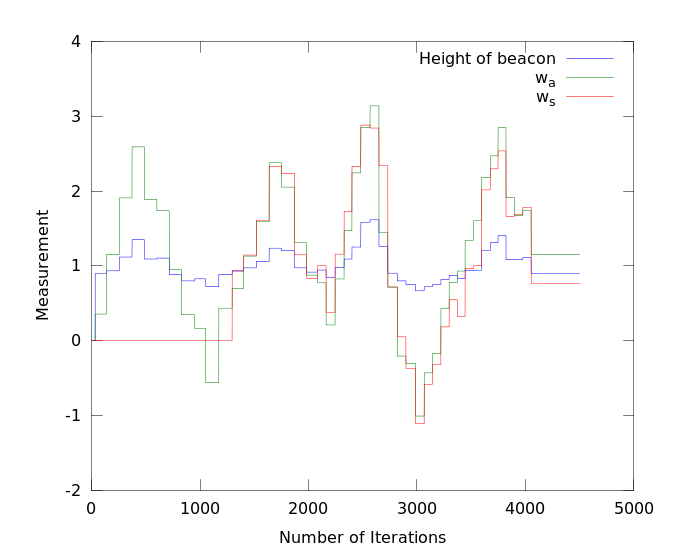
\includegraphics[width=0.7\columnwidth]{out_obs.png}
\caption{Testing of ASAMI on Nao. The observation comes only when it's
in standing phase. So there is less update in the observation, and
less noise compared to Figre~\ref{fig:demo}. One iteration of ASAMI
corresponds to one update in the figure, which corresponding to many
frames on Nao (I re-scaled the height of beacon, so that they can be
plotted in a same magnitude).}
\label{fig:obs}
\end{figure}

I later realized that making Nao observe while walking is not
necessary (though interesting). So I made the Nao observe only when
standing.  The performance is that, the Nao takes an action, and then
walk, and then stands still to look at the beacon. It keeps repeating
this sequence. The result is in Figure~\ref{fig:obs}.  The height of
beacon in the figure is the average of the observed beacon heights in
the standing phase. Note that the x label in Figure~\ref{fig:obs} is
different from that in Figure~\ref{fig:demo}. In Figure~\ref{fig:demo},
one iteration of ASAMI is exactly one frame on Nao. Here, one
iteration of ASAMI takes many frames on Nao (one walking and one
standing phase).

Clearly, as there are less noise in the observation, ASAMI has a
better learning performance.

\subsection{Test on Nao: using Strong ASAMI}

\begin{figure}[h]
\centering
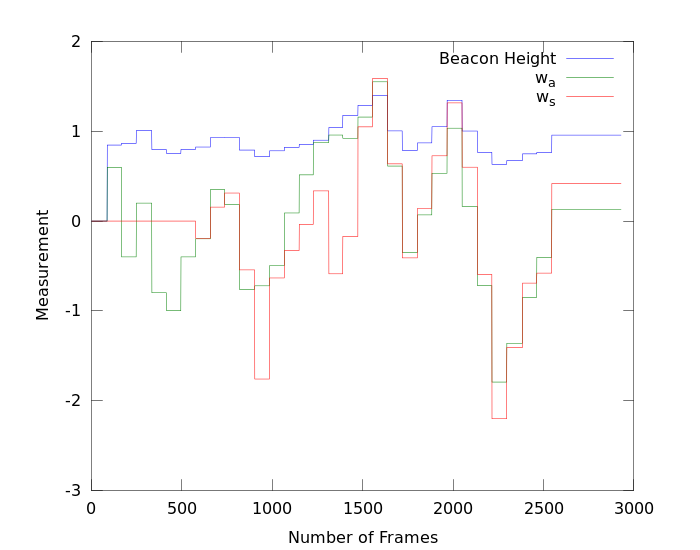
\includegraphics[width=0.7\columnwidth]{out_strong.png}
\caption{Testing of Strong ASAMI on Nao. The observation comes only
when it's in standing phase - same as Figure~\ref{fig:obs}. The robot
tries to learn the action model first in the first 1,500 iterations,
then continues to explore the state space (I re-scaled the height of
beacon, so that they can be plotted in a same magnitude).}
\label{fig:obs_strong}
\end{figure}

Strong ASAMI is applied in this experiment. The assumption is
different from the previous ones - Nao doesn't have the knowledge of
the actions. The results are in Figure~\ref{fig:obs_strong}. It can be
told from the beacon height that the robot tries different actions
first (within 1,500 iterations, or frames) and then move forward and
backward to explore the state space.

Another intended goal is to show that convergence in
Figure~\ref{fig:obs_strong} should be faster than that in previous
experiments. Actually, the difference is not significant, at least for
one-dimensional environment.

\section{Discussion and Conclusion}
\label{sec:dis}

It is possible that learning each discrete action independently would
have a better performance. That would be the same metric as
\cite{LNAI2007-ahmadi}. Though it is interesting to estimate what
the most likely continuous model is, expressed by polynomial function.
It has several constraints. First, degree selection should be
determined, possibly using methods in \cite{IJAIT08-stronger}. But the
model may not be a small-dimensional polynomial, so there might be
too many parameters to estimate. Second, the inherent drawback of
function approximation method is that local updates could have global
effects. This is especially harmful in a noisy environment.

The idea of action trials is very similar to the idea of N-bandit
problem \cite{vermorel2005multi}. Though we are not going to find an
optimal action. The goal should be the smallest variance of all the
actions. To solve this problem, I used a very naive approach - always
choosing an action with the least variance. However, the actions are
not mutually independent - they are picked up from a continuous space.
So getting one sample of an action can help us know its neighborhood.

The action model and sensor model are comparatively easy to learn for
a one-dimensional environment. So expecting improvement based on the
result of ASAMI algorithm may not be realistic. However, Strong ASAMI
does show its power in the environment where action learning is
necessary.

%=====================================================================
\bibliographystyle{plain}

\bibliography{report}

\end{document}
